% Package
\documentclass[11pt]{article}

\usepackage{amsmath}
\usepackage{cite}
\usepackage{graphicx}
\usepackage[utf8]{inputenc}
\usepackage[T1]{fontenc}
\usepackage{lmodern}

\title{ADP Aufgabe 1, Abgabe 1}
\author{Team 1\\Hugo Protsch, Justin Hoffmann}

% Document
\begin{document}

    \maketitle


    \section{Formales}\label{sec:Formales}

    %! suppress = MissingLabel

    \subsection{Aufgabenaufteilung}
    Die Entwürfe wurden zusammen entwickelt.
    %! suppress = MissingLabel

    \subsection{Quellenangaben}
    
    Es wurden lediglich Vorlesungsmaterialien verwendet.

    %! suppress = MissingLabel

    \subsection{Bearbeitungszeitraum}
    Für die Bearbeitung haben wir in etwa 8 bis 10 Stunden benötigt.
    %! suppress = MissingLabel

    \subsection{Aktueller Stand}
    Der Entwurf ist nach erhaltenem Feedback überarbeitet und fertiggestellt.

    %! suppress = MissingLabel

    \subsection{Änderungen des Entwurfes}
    InitBT ist nicht mehr "trivial" und besitzt nun ein eigenes Ablaufdiagramm mit Erläuterungen.
    
    In IsBT wird nun spezifiziert, wie ein "Blatt" auszusehen hat.
    
    Die Sortierung in IsBT wird nun durch dynamische Intervalle überprüft.
    
    EqualBT ist nicht mehr "trivial" und besitzt  nun ein eigenes Ablaufdiagramm mit Erläuterungen.
    
    Die Frage, ob ein Baum "existiert" wurde an allen vorkommenden Stellen im Entwurf überarbeitet zu der Frage, ob "ein Baum leer ist".
    
    Hilfsfunktion findAndDelete inkl. Ablaufdiagramm und Erläuterungen hinzugefügt.
    
    Löschvorgang von DeleteBT bzw. findAndDelete konkretisiert.
    
    Laufzeitanalyse wird nun im Detail durch einen eigenen Testentwurf beschrieben.


    \section{Entwürfe}\label{sec:entwuerfe}

    \subsection{InitBT}\label{subsec:initbt}
    
    \begin{center}
        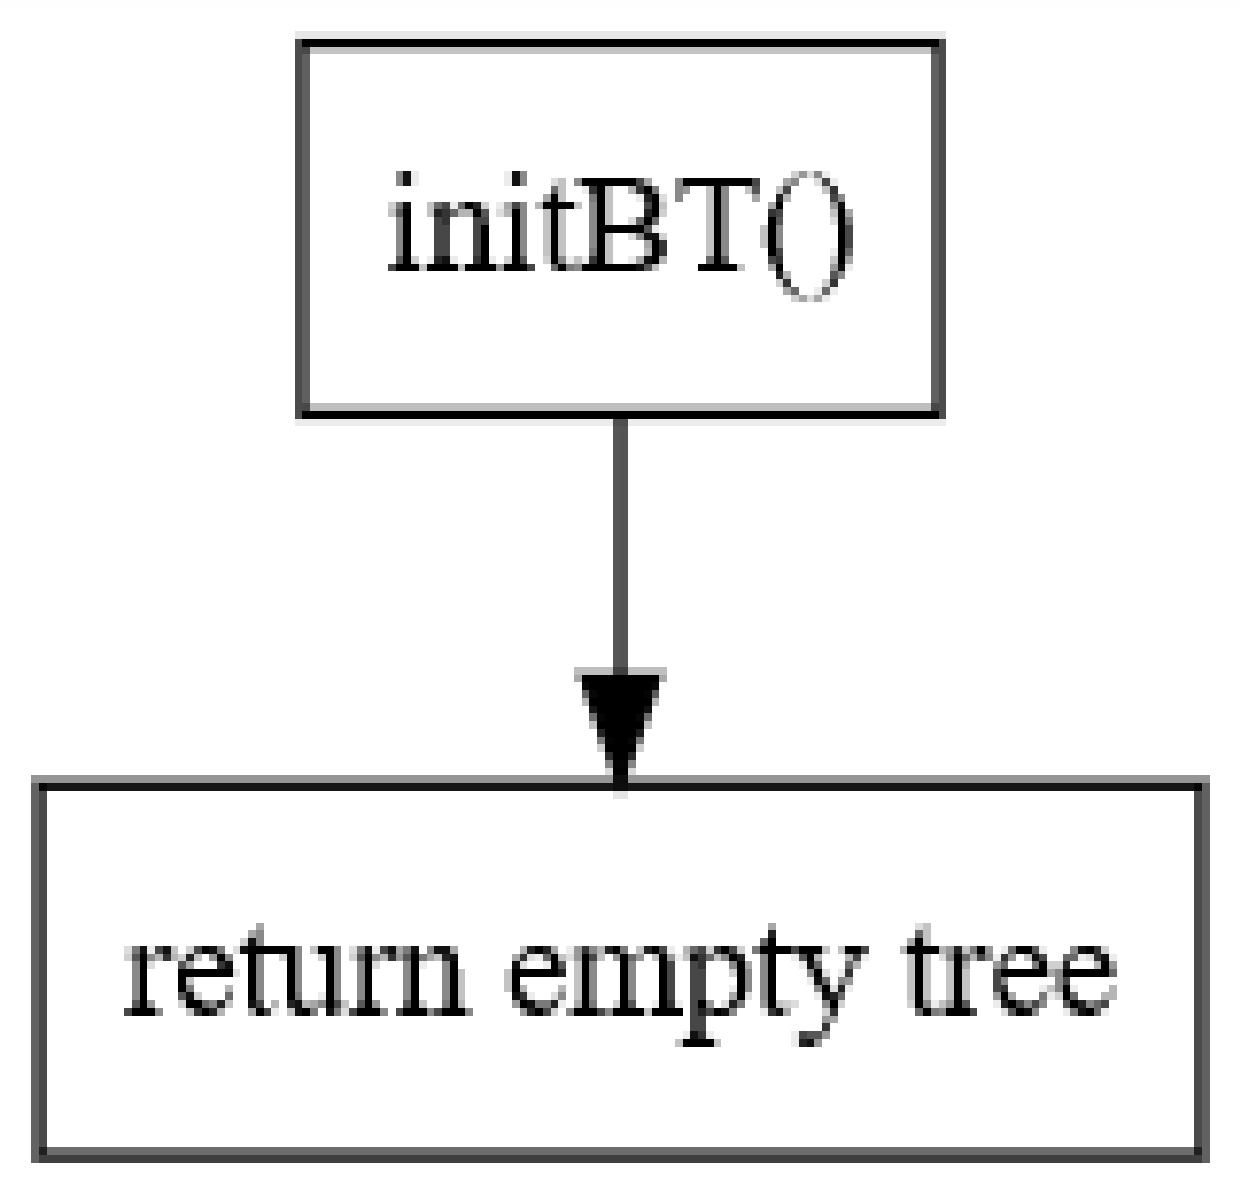
\includegraphics[width=0.2\columnwidth] {init.pdf}
    \end{center}
    
    Liefert einen leeren Baum.
    Die erwartete Laufzeit beträgt
    \begin{math}
        \Theta(1)
    \end{math}

    \subsection{IsEmptyBT}\label{subsec:isemptybt}
    
    \begin{center}
        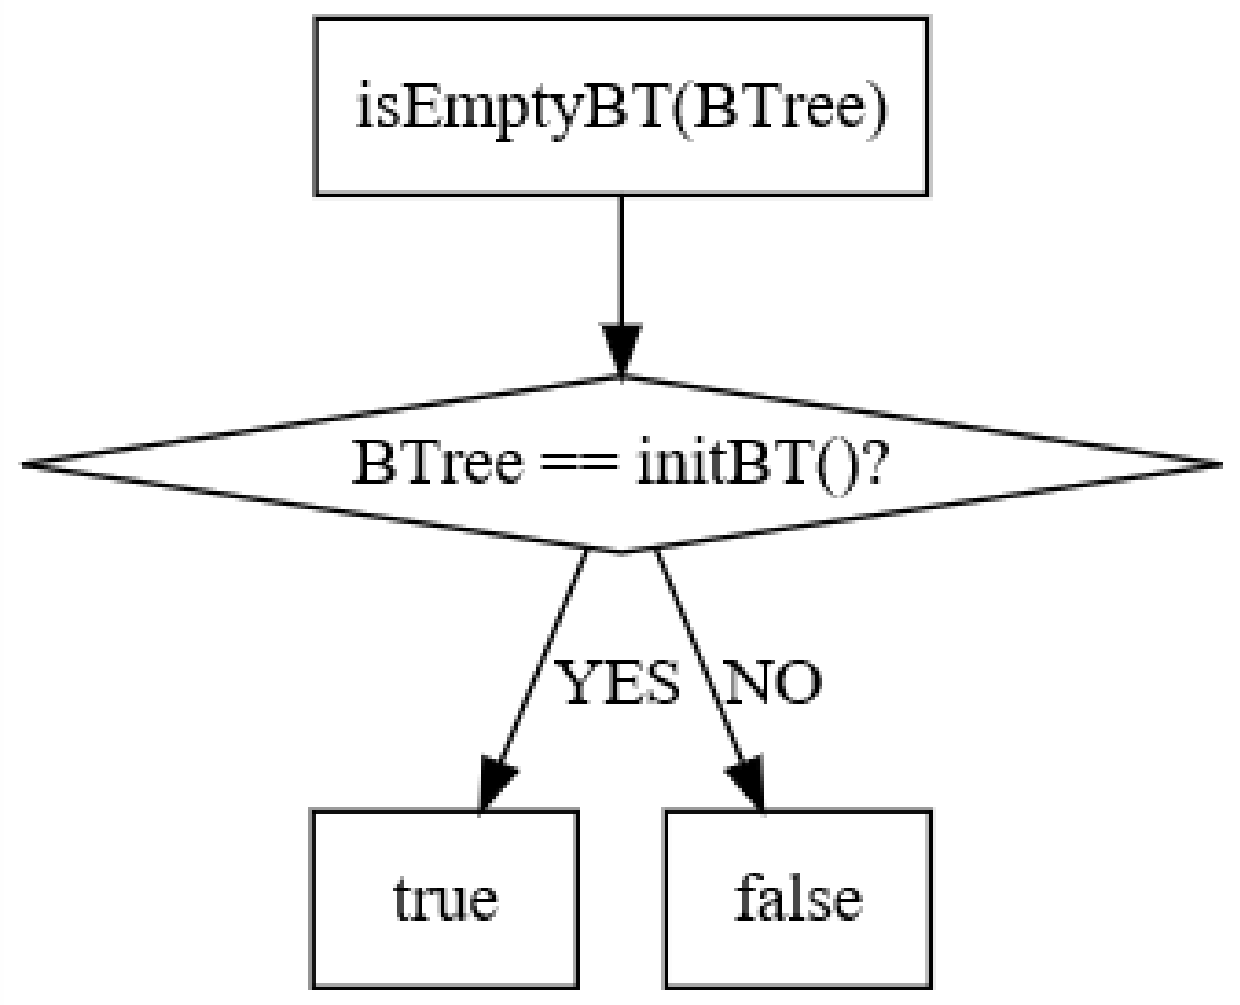
\includegraphics[width=0.39\columnwidth] {isempty.pdf}
    \end{center}
    
    Prüft einen Baum auf Leerheit.
    Dies erfolgt durch einen Vergleich mit dem Resultat von
    initBT. Liefert dieser true ist der Baum leer, bei false
    nicht.

    Die erwartete Laufzeit beträgt
    \begin{math}
        \Theta(1)
    \end{math}

    \subsection{IsBt}\label{subsec:isbt}

    \begin{center}
        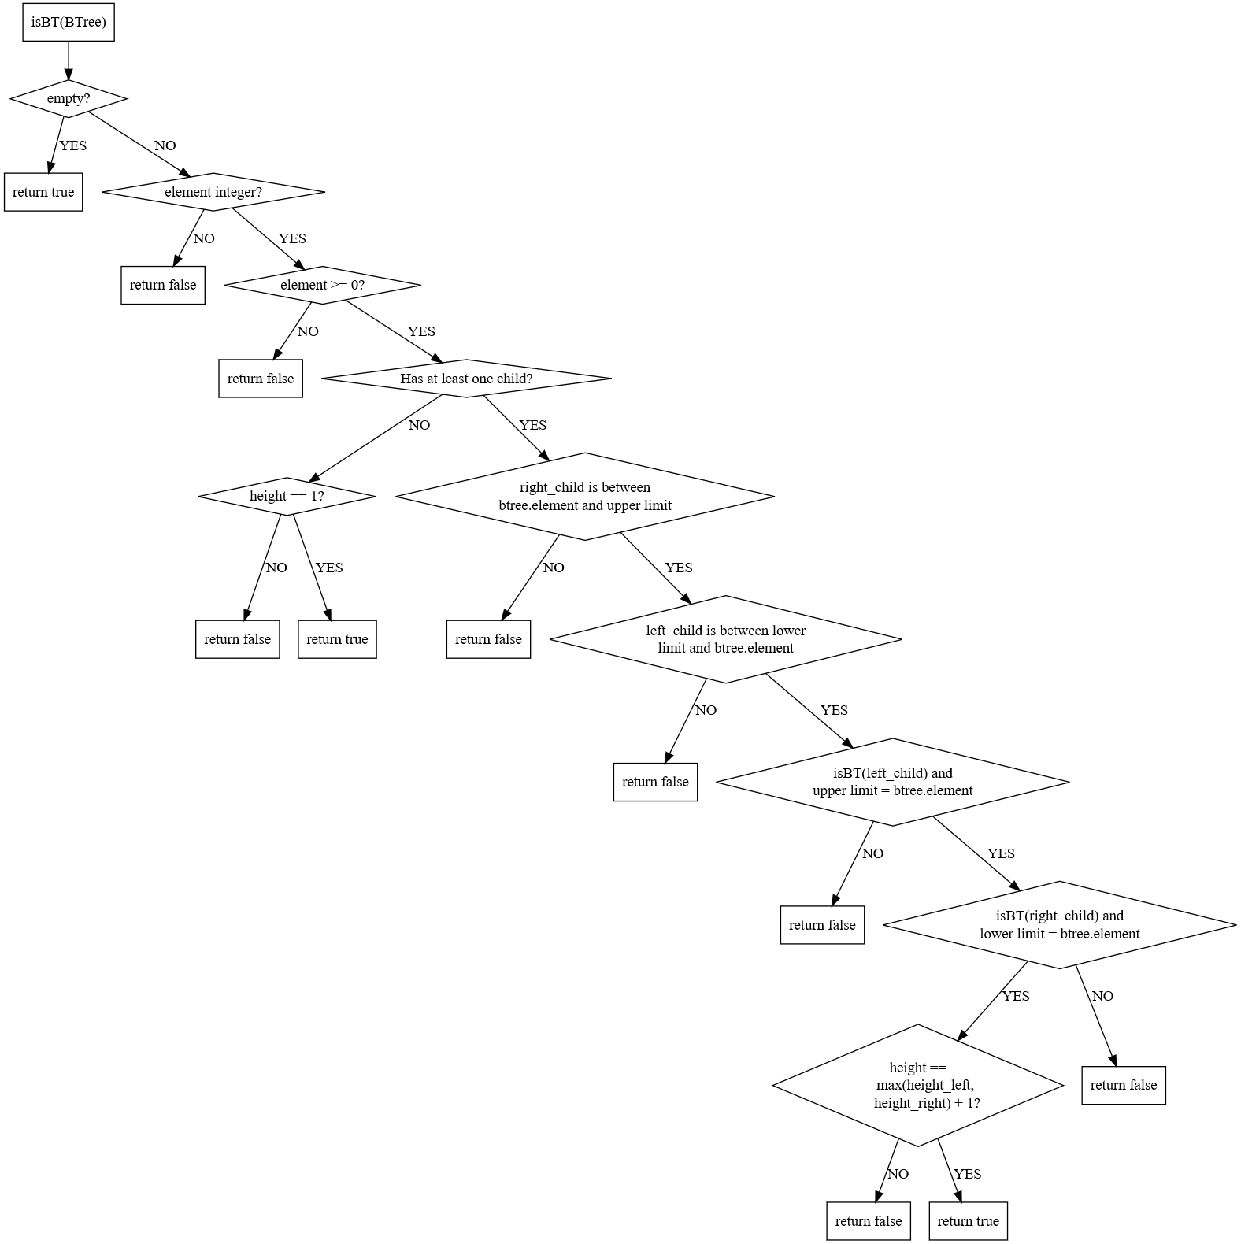
\includegraphics[width=1.2\columnwidth] {isbt.pdf}
    \end{center}

    Prüft die vorgegebenen Rahmenbedingungen eines übergebenen Baums.
    Die Sortierung der Elementwerte innerhalb des Bäumes wird hierbei mit einer oberen und unteren Grenze, die dynamisch angepasst wird sichergestellt. Im Default-Fall wertet die obere Grenze zu etwas aus, was größer als jeder Integer ist und die untere Grenze zu dem größten nicht erlaubten Wert.
    Alle Wahrheitswerte der verschiedenen
    Vorgaben von jedem Knoten werden miteinander in einen logischen
    Zusammenhang gebracht.

    Die erwartete Laufzeit beträgt
    \begin{math}
        O(n)
    \end{math}

    \subsection{EqualBT}\label{subsec:equalbt}
    
    \begin{center}
        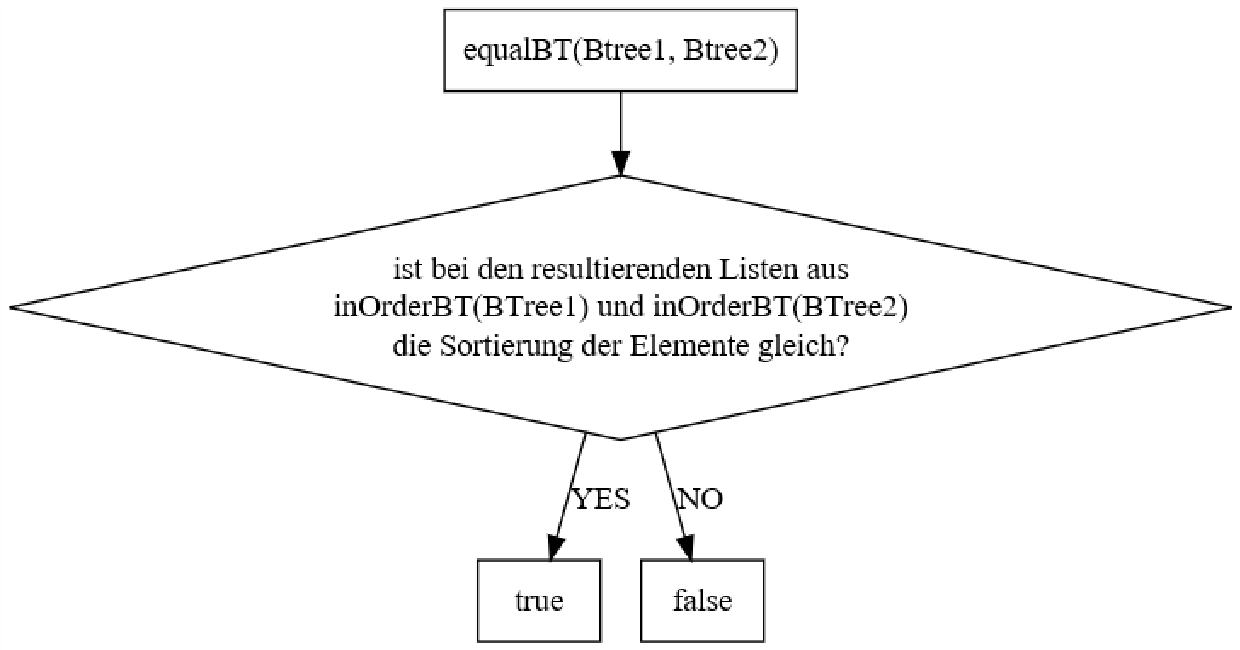
\includegraphics[width=0.7\columnwidth] {equal.pdf}
    \end{center}
    
    Prüft auf semantische Gleichheit zwischen zwei Bäumen.
    Zuerst werden mit inOrderBT beide Bäume als sortierte Listen ausgegeben,
    Anschließend wird elementweise auf Gleichheit geprüft.
    Die resultierenden Listen sind gleich wenn die Reihenfolgen der Elemente gleich sind.
    Falls die Listen gleich sind, wird true zurückgegeben, sonst false.

    Die erwartete Laufzeit beträgt
    \begin{math}
        O(n)
    \end{math},
    da die Bäume unabhängig voneinander durchlaufen werden, im Anschluss wird
    ein Mal über eine Liste von n Elementen iteriert.

    \subsection{InsertBT}\label{subsec:insertbt}

    \begin{center}
        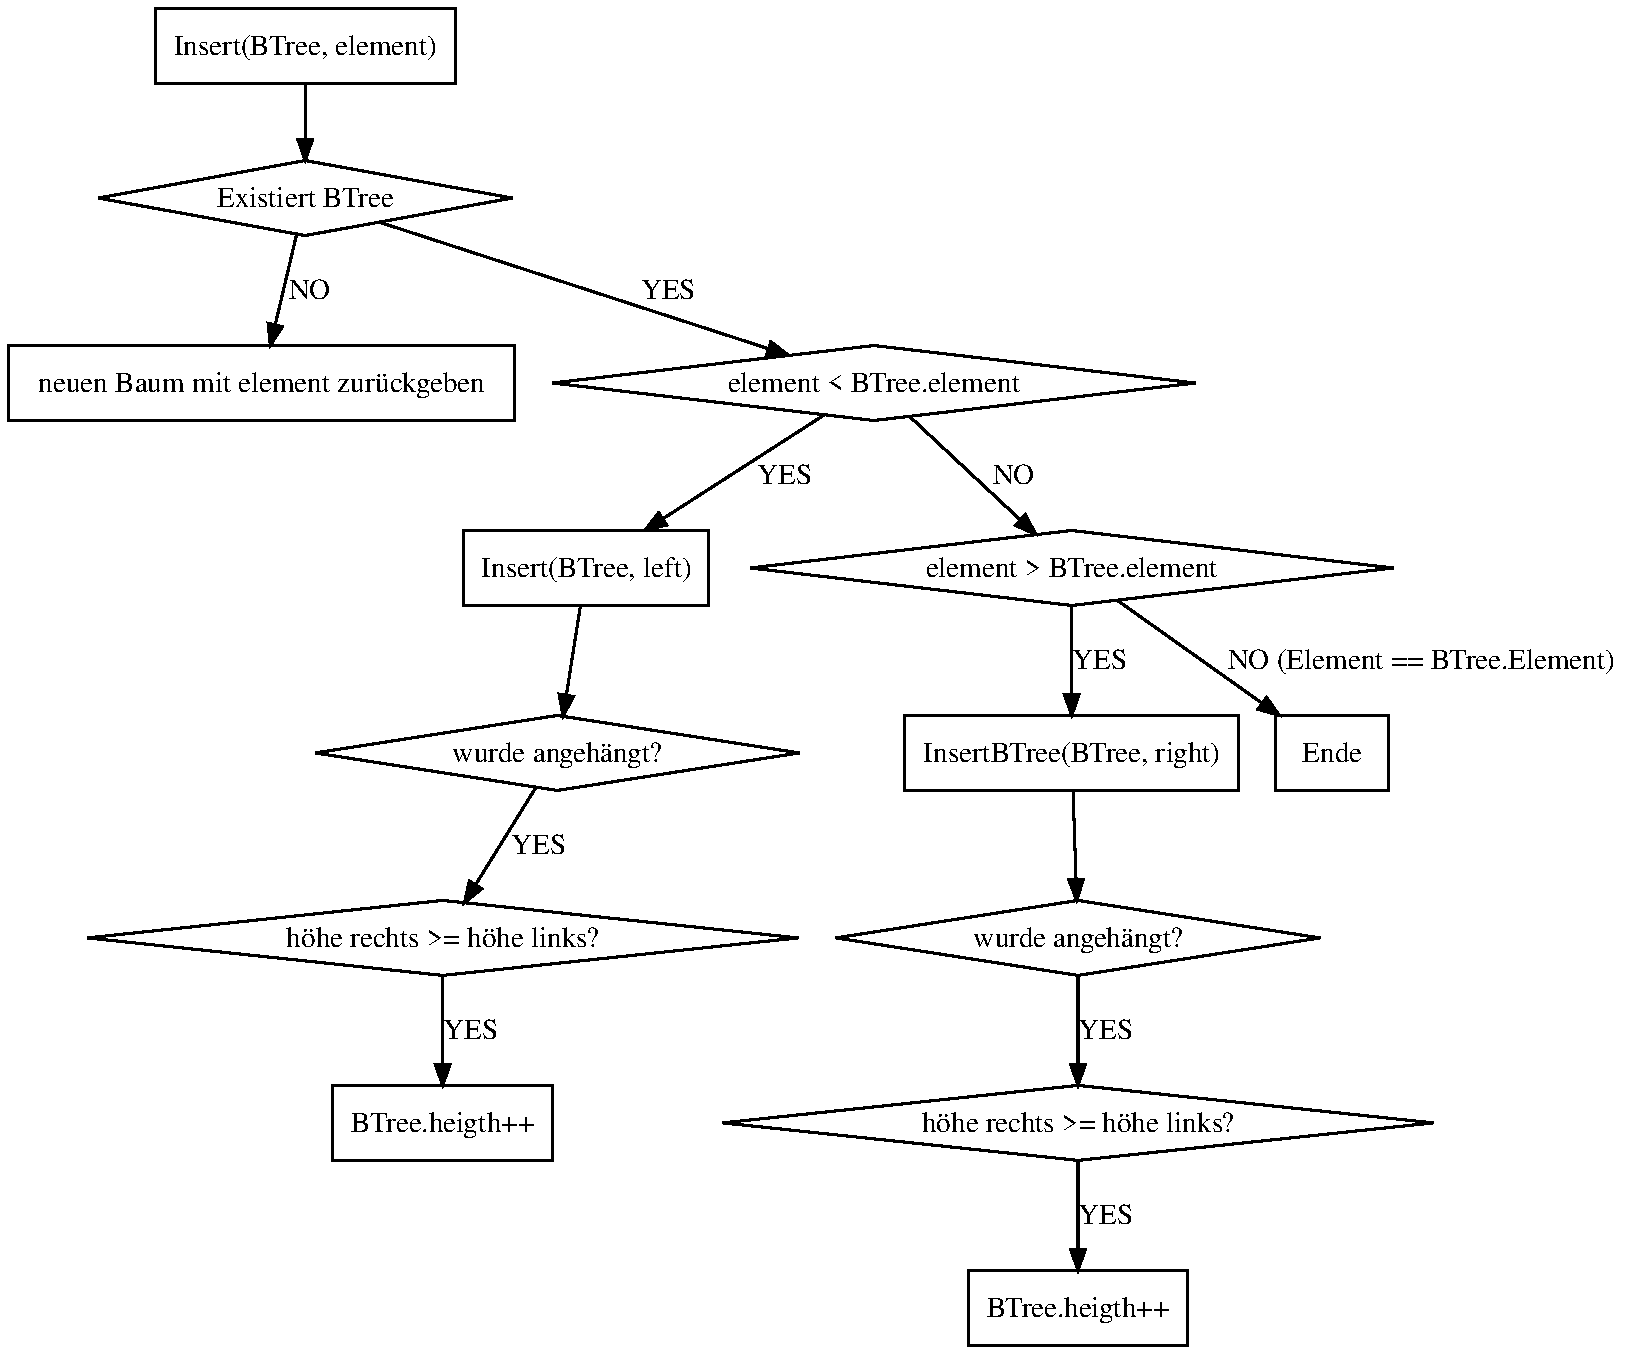
\includegraphics[width=1.1\columnwidth] {insert.pdf}
    \end{center}

    Fügt ein übergebenes Element einem übergebenem Baum hinzu.
    Zum Traversieren des Baumes wird bei jedem Schritt überprüft,
    ob das einzufügende Element kleiner oder größer dem derzeitigen Knoten-Element ist.
    Ist es kleiner, geht man nach links, größer nach rechts.
    Wenn bereits ein Knoten mit dem gleichen Wert existiert, wird der Baum
    unverändert zurückgegeben.
    Wurde ein leerer Platz gefunden, wird das Element dort eingefügt.
    Die Höhe wird in jedem Knoten bottom-up mithilfe der Definition der Höhe neu berechnet. Das Größere der beiden Kindelemente wird um 1 addiert. So wird die Integrität der Höhe sichergestellt.


    Die erwartete Laufzeit beträgt
    \begin{math}
        O(n)
    \end {math}
    bzw.
    \begin{math}
        \Theta (log (n))
    \end{math},
    da der Baum im Worst-Case nicht ausgeglichen ist.
    Das hat zur Folge, dass alle Elemente einmal durchlaufen werden müssen.
    Durchschnittlich wird der Baum mit einer logarithmischen Komplexität
    traversiert, da bei einem ausgeglichenem Baum durch die vertikale
    Traversierung nur
    \begin{math}
        log (n)
    \end{math}
    Elemente durchlaufen werden.

    \subsection{DeleteBT}\label{subsec:deletebt}

    \begin{center}
        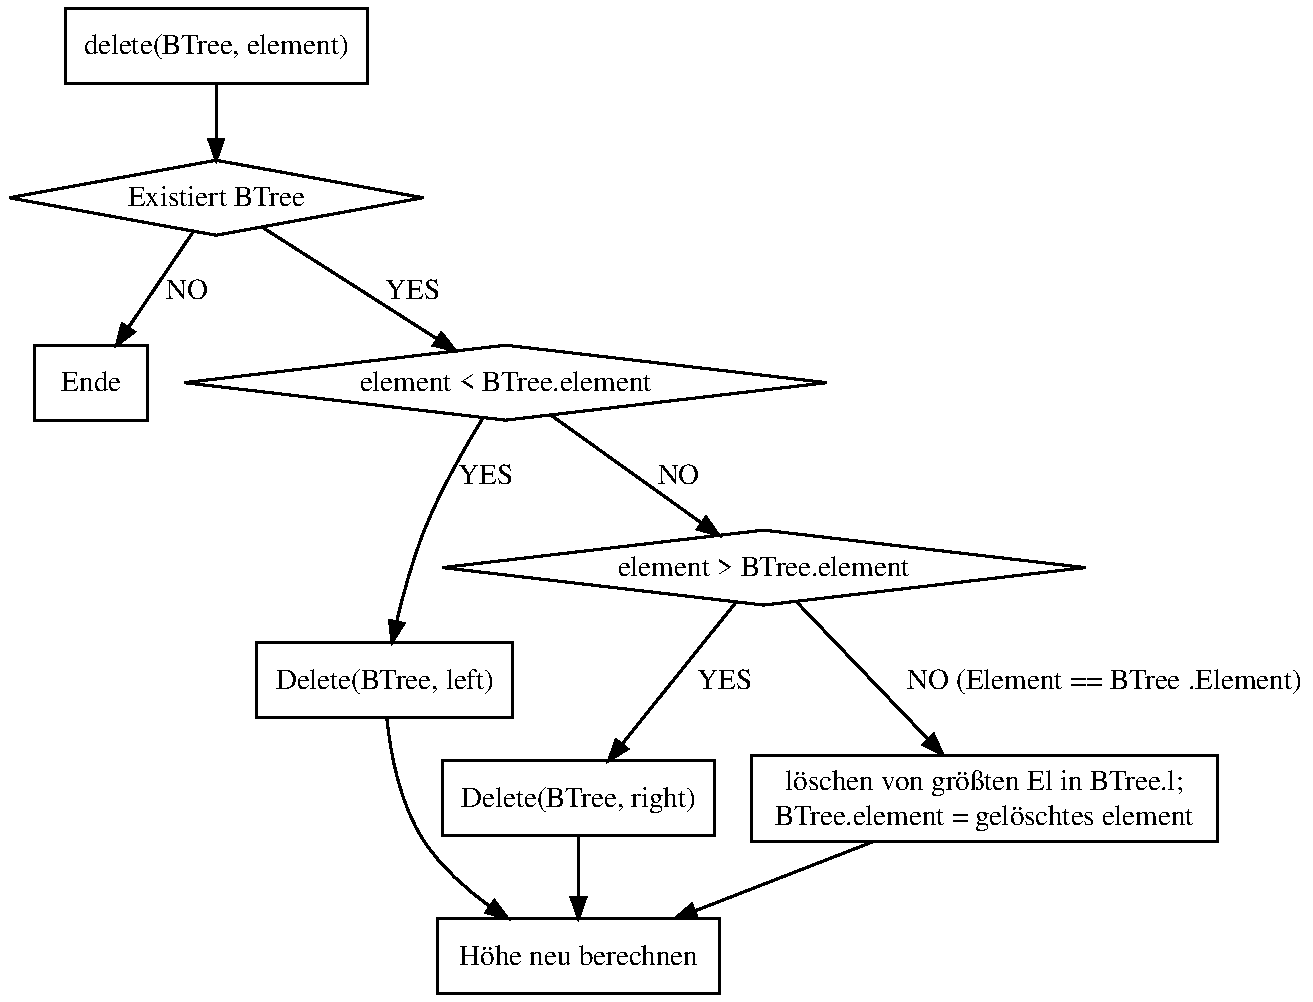
\includegraphics[width=0.8\columnwidth] {delete.pdf}
    \end{center}

    Löscht ein übergebenes Element aus einem übergebenem Baum.
    Die Traversierung des Baums ist gleich wie bei InsertBT.
    Ist das Ende des Baumes erreicht, ohne das Element gefunden zu haben,
    wird der Baum unverändert zurückgegeben.
    Wird das Element aufgefunden, folgt der Aufruf einer Hilfsfunktion findAndDeleteMax, die das größte Element aus dem linken Baum löscht und zurückgibt. Das Element, das gelöscht werden soll wird nun durch das gefundene Element ersetzt. Die Höhe wird wieder bottom-up laut Definition angepasst.

    Die erwartete Laufzeit beträgt
    \begin{math}
        O(n)
    \end {math}
    bzw.
    \begin{math}
        \Theta (log (n))
    \end{math}
    aufgrund der bei InsertBT erwähnten Umstände.
    
    
    \subsection{findAndDeleteMax}\label{subsec:findanddeletemax}

    \begin{center}
        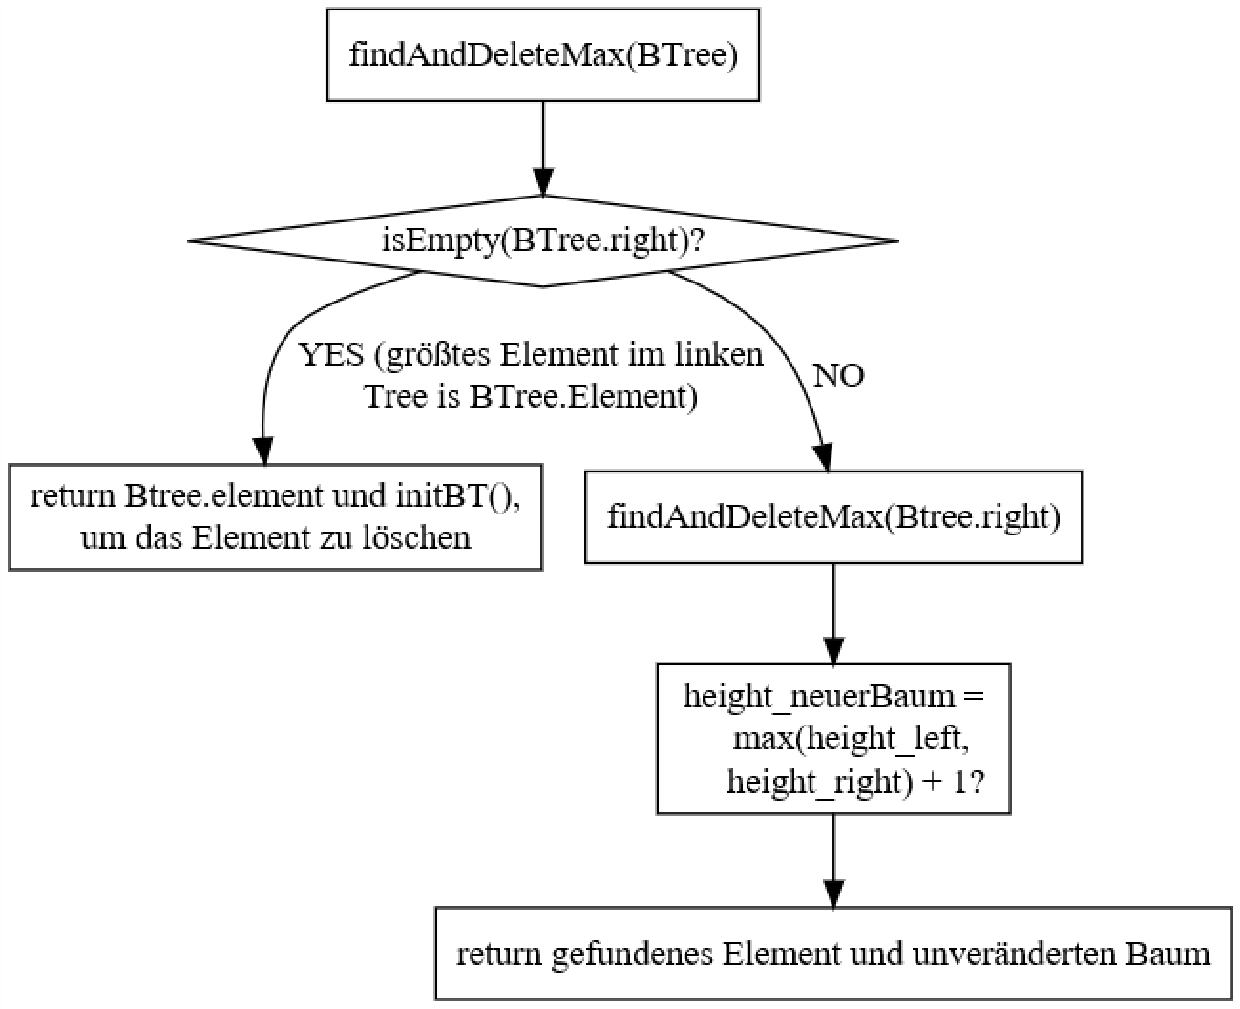
\includegraphics[width=0.65\columnwidth] {findanddeletemax.pdf}
    \end{center}

    Löscht das größte Element aus einem übergebenem Baum und gibt dieses, zusammen mit dem neuen Baum, zurück. Das tatsächliche Löschen des größten Elements erfolgt durch das zurückgeben des leeren Baumes sobald dieses gefunden wird. Auch hier wird die Höhe bottom-up berechnet.

    Die erwartete Laufzeit beträgt
    \begin{math}
        O(n)
    \end {math}
    bzw.
    \begin{math}
        \Theta (log (n))
    \end{math}
    mit einer ähnlichen Begründung wie von InsertBT bzw. DeleteBT, da der Baum lediglich von dem Punkt aus, in dem die Funktion aufgerufen wird bis nach unten traversiert.
    

    \subsection{Find}\label{subsec:find}

    \begin{center}
        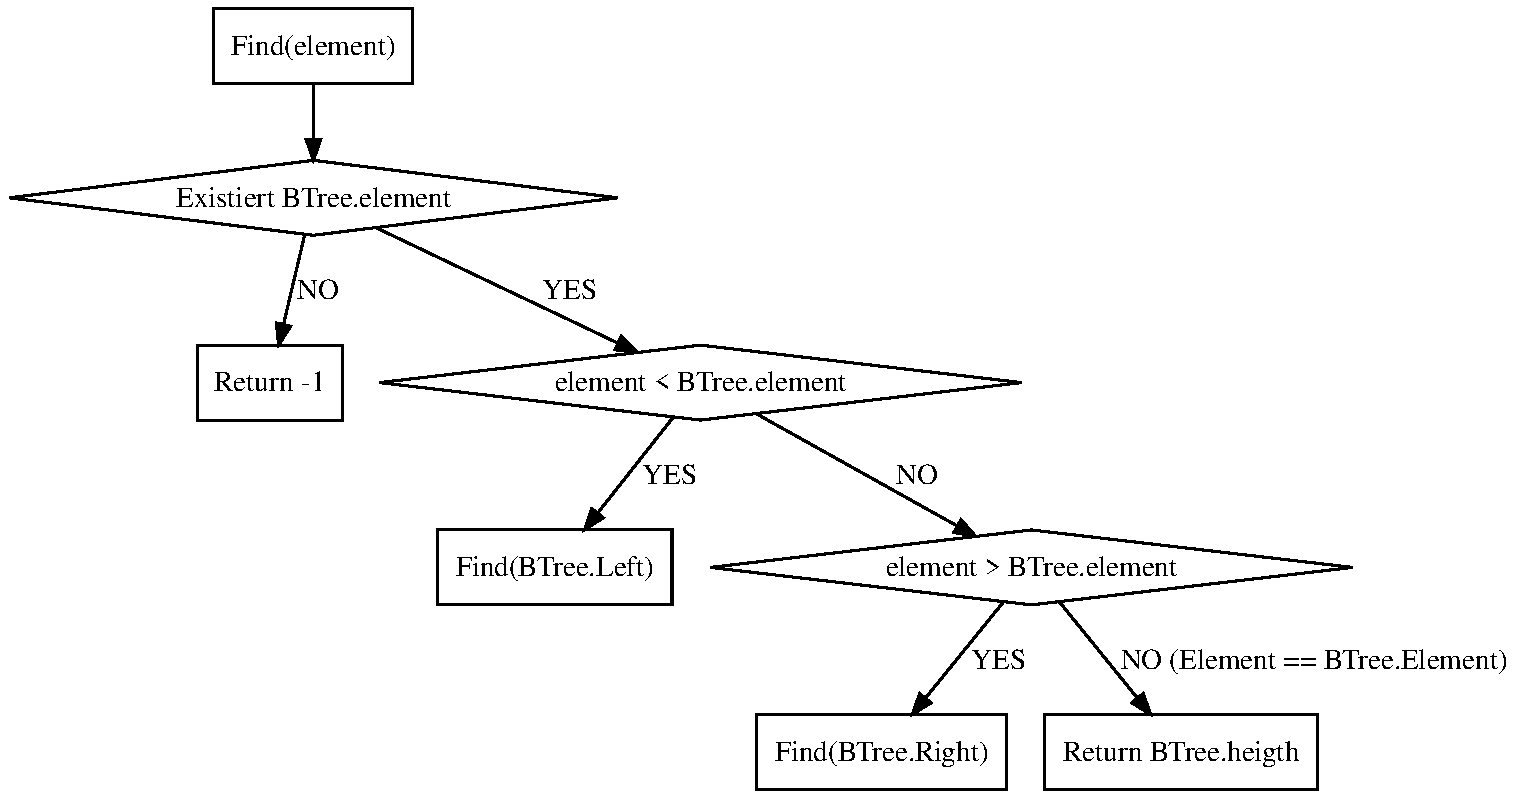
\includegraphics[width=1.1\columnwidth] {find.pdf}
    \end{center}

    Gibt die Höhe eines übergebenem Elements in einem übergebenem Baum aus.
    Traversieren des Baums funktioniert hierbei gleich wie in InsertBT.
    Ist das Element gefunden, wird die Höhe des Knotens ausgegeben.

    Die erwartete Laufzeit beträgt
    \begin{math}
        O(n)
    \end {math}
    bzw.
    \begin{math}
        \Theta (log (n))
    \end{math}
    aufgrund der bei InsertBT erwähnten Umstände.

    \subsection{InOrderBT}\label{subsec:inorderbt}

    \begin{center}
        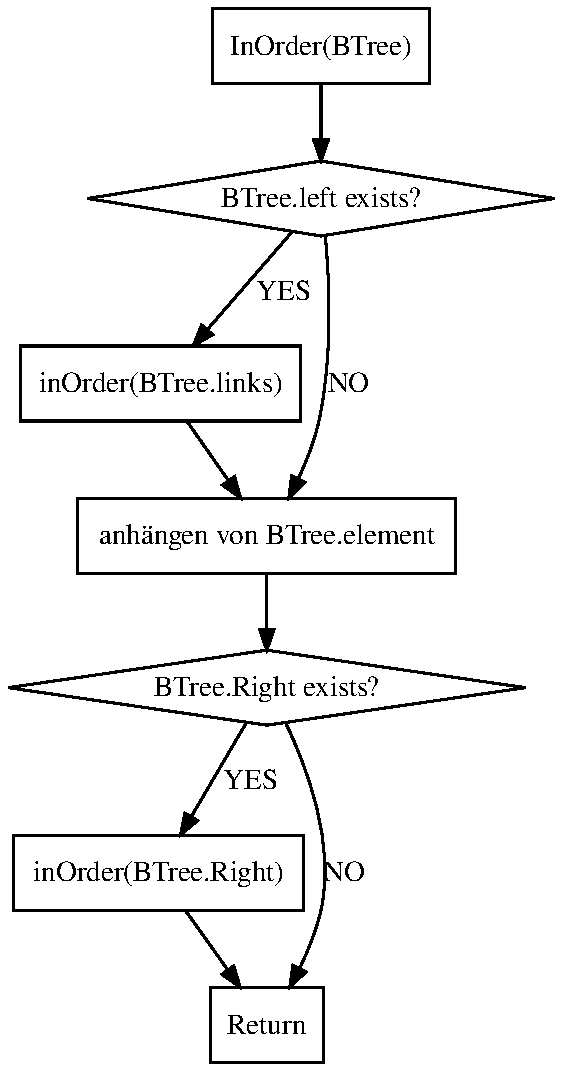
\includegraphics[width=0.4\columnwidth] {inorderhugo.pdf}
        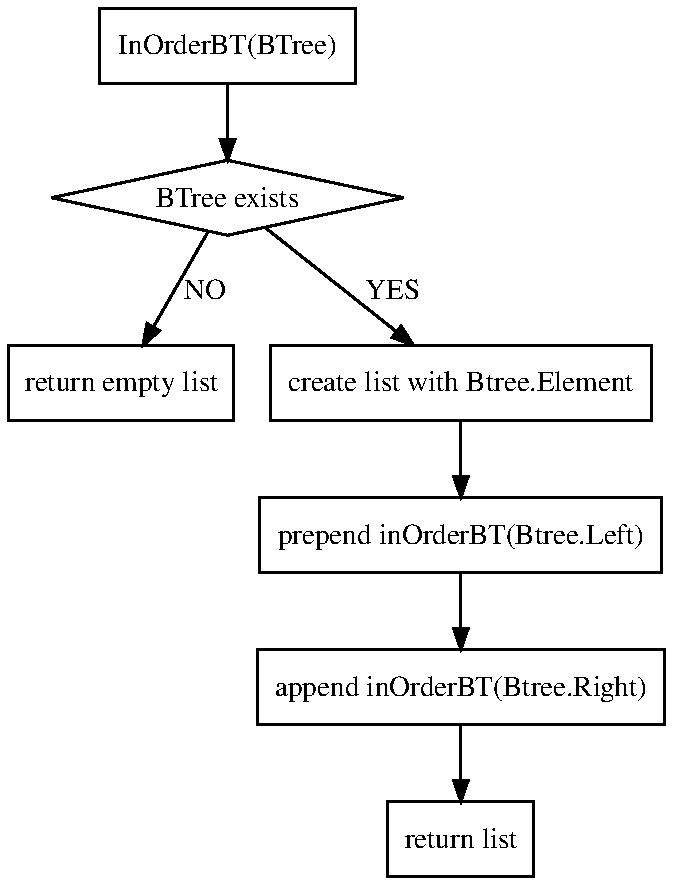
\includegraphics[width=0.5\columnwidth] {inorderjustin.pdf}
    \end{center}

    Gibt den Baum in Inorder in einer Liste aus.
    Es wird eine Liste mit dem Element des Knotens erstellt,
    wobei die Inorder des linken Kindes vorangestellt und die
    Inorder des rechten Kindes herangehängt wird.
    Ist das Ende des Baumes erreicht, wird eine leere Liste zurückgegeben.

    Hier haben wir zwei Optionen dargestellt: Zum Einen kann bei jedem
    Funktionsdurchlauf der derzeitige Knoten selbst betrachtet werden (rechts).
    Zum anderen gibt es die Möglichkeit, vorausschauend zu arbeiten und immer
    auf die Kinder des derzeitigen Knotens achten (links).
    Die Auswahl des Entwurfes ist implementationsabhängig.

    Die erwartete Laufzeit beträgt
    \begin{math}
        \Theta (n)
    \end{math},
    da jedes Element des Baums durchlaufen wird.
    Hierbei ist zu beachten, dass die Gesamtkomplexität des Weiteren von der
    Komplexität der Append- bzw. Prepend-Operation der Liste abhängt.
    Falls die Komplexität dieser Operation
    \begin{math}
        O(n)
    \end{math}
    beträgt, ergibt sich daraus eine Gesamtkomplexität von
    \begin{math}
        O(log(n) \cdot n)
    \end{math}


    \section{Laufzeitmessung}\label{sec:laufzeitmessung}

    Für den Versuch der Laufzeitmessung werden jeweils die Funktionen mit
    variierender Elementanzahl getestet. Beginnend bei
    annähernd 0 Elementen wird die Anzahl jeweils um eine feste Schrittgröße
    erhöht. Hierbei ist das Ziel, die Schrittgröße so zu wählen, dass bei 20
    Schritten eine maximale Laufzeit von ca. 5 Sekunden (5000ms) erreicht
    wird. Wir mitteln über 3 Durchgänge.
    Falls die Abweichungen zwischen den Durchgängen zu groß sind, kann die
    Anzahl der dieser nachträglich angepasst werden.

    Es werden drei Messungen, eine mit zufälligen, eine mit
    aufsteigenden und eine mit absteigenden Zahlen, ausgeführt.
    Bei absteigenden und aufsteigenden Zahlen erwarten wir jeweils den
    Worst-Case, bei zufälligen den Average-Case.

    Die Laufzeit wird anschließend mit besagter Eingangsgröße in Relation gesetzt.
    Wir vergleichen den gemessenen funktionellen Zusammenhang mit dem Erwarteten,
    welcher in den Entwürfen der jeweiligen Funktion beschrieben ist.

    Die Rahmenbedingungen der Messung sind hierbei vorgegeben.

\end{document}
